\documentclass[11pt]{article}

% some definitions for the title page
\newcommand{\reporttitle}{RNN and Attention}
\newcommand{\reportdescription}{}

% load some definitions and default packages
%---------------------------------------------------------------------------
%	PACKAGES AND OTHER DOCUMENT CONFIGURATIONS
%---------------------------------------------------------------------------

\usepackage[twoside]{fancyhdr}
\usepackage{csquotes}

\usepackage[a4paper,hmargin=2.0cm,vmargin=1.0cm,includeheadfoot]{geometry}
% \usepackage{natbib} % for bibliography
\usepackage{biblatex}
\usepackage{tabularx,longtable,multirow,subfigure,caption}%hangcaption
\usepackage{fancyhdr} % page layout
\usepackage{url} % URLs
\usepackage[english]{babel}
\usepackage{graphicx}
\usepackage{rotating}
\usepackage{dsfont}
\usepackage{epstopdf} % automatically replace .eps with .pdf in graphics
% \usepackage{backref} % needed for citations
\usepackage{array}
\usepackage{latexsym}
\usepackage[pdftex,hypertexnames=false,colorlinks]{hyperref} % provide links in pdf (had pagebackref)
\usepackage{booktabs}
\usepackage{wrapfig}
\usepackage{caption}  % Required for \captionof
\usepackage{float} % for H option in figures
\usepackage{amssymb}
\usepackage{amsmath}
\usepackage{amsthm}
\usepackage{mathtools} % for 'dcases*' env.
\usepackage[nottoc]{tocbibind}

%%% Default fonts
\renewcommand*{\rmdefault}{bch}
\renewcommand*{\ttdefault}{cmtt}

%%% Default settings (page layout)
\setlength{\parindent}{0em}  % indentation of paragraph
\setlength{\parskip}{.3em}
\setlength{\itemsep}{0.mm}

\setlength{\headheight}{14.5pt}
\pagestyle{fancy}

\fancyfoot[ER,OL]{\thepage}%Page no. in the left on odd pages and on right on even pages

\fancyfoot[OC,EC]{\sffamily }
\renewcommand{\headrulewidth}{0.1pt}
\renewcommand{\footrulewidth}{0.1pt}
\captionsetup{margin=10pt,font=small,labelfont=bf}

% LISTINGS ammendments
\usepackage{listings}
\usepackage{color}

\definecolor{mygreen}{rgb}{0,0.6,0}
\definecolor{mygray}{rgb}{0.5,0.5,0.5}
\definecolor{mymauve}{rgb}{0.58,0,0.82}

\lstset{ 
  postbreak=\mbox{\textcolor{red}{$\hookrightarrow$}\space},
  backgroundcolor=\color{white},   % choose the background color; you must add \usepackage{color} or \usepackage{xcolor}; should come as last argument
  basicstyle=\footnotesize,        % the size of the fonts that are used for the code
  breakatwhitespace=false,         % sets if automatic breaks should only happen at whitespace
  breaklines=true,                 % sets automatic line breaking
  captionpos=b,                    % sets the caption-position to bottom
  commentstyle=\color{mygreen},    % comment style
%   deletekeywords={...},            % if you want to delete keywords from the given language
%   escapeinside={\%*}{*)},          % if you want to add LaTeX within your code
  extendedchars=true,              % lets you use non-ASCII characters; for 8-bits encodings only, does not work with UTF-8
  firstnumber=1,                % start line enumeration with line 1000
  frame=single,	                   % adds a frame around the code
  keepspaces=true,                 % keeps spaces in text, useful for keeping indentation of code (possibly needs columns=flexible)
  columns=fullflexible,
  keywordstyle=\color{blue},       % keyword style
  language=python,                 % the language of the code
  % morekeywords={*,...},            % if you want to add more keywords to the set
  numbers=left,                    % where to put the line-numbers; possible values are (none, left, right)
  numbersep=5pt,                   % how far the line-numbers are from the code
  numberstyle=\tiny\color{mygray}, % the style that is used for the line-numbers
  rulecolor=\color{black},         % if not set, the frame-color may be changed on line-breaks within not-black text (e.g. comments (green here))
  showspaces=false,                % show spaces everywhere adding particular underscores; it overrides 'showstringspaces'
  showstringspaces=false,          % underline spaces within strings only
  showtabs=false,                  % show tabs within strings adding particular underscores
  stepnumber=1,                    % the step between two line-numbers. If it's 1, each line will be numbered
  stringstyle=\color{mymauve},     % string literal style
  tabsize=2,	                   % sets default tabsize to 2 spaces
  title=\lstname% show the filename of files included with \lstinputlisting; also try caption instead of title
}

% Here, you can define your own macros. Some examples are given below.

\newcommand{\R}[0]{\mathds{R}} % real numbers
\newcommand{\Z}[0]{\mathds{Z}} % integers
\newcommand{\N}[0]{\mathds{N}} % natural numbers
\newcommand{\C}[0]{\mathds{C}} % complex numbers
\renewcommand{\vec}[1]{{\boldsymbol{{#1}}}} % vector
\newcommand{\mat}[1]{{\boldsymbol{{#1}}}} % matrix


%\bibliography{bibliography}

\begin{document}

% Include the title page
\begin{titlepage}

    \newcommand{\HRule}{\rule{\linewidth}{0.5mm}} % Defines a new command for the horizontal lines, change thickness here
    
    \center % Center everything on the page
     
    %------------------------------------------------------------------------
    %	HEADING SECTIONS
    %------------------------------------------------------------------------
    
    \textsc{\Large Department of Computing}\\[0.5cm] 
    \textsc{\large Imperial College of Science, Technology and Medicine}\\[0.5cm] 
    
    %------------------------------------------------------------------------
    %	TITLE SECTION
    %------------------------------------------------------------------------
    
    \HRule \\[0.4cm]
    { \huge \bfseries \reporttitle}\\ % Title of your document
    \HRule \\[0.4cm]

    \textit{\reportdescription}
    
    \vspace{2em}

    %------------------------------------------------------------------------
    %	AUTHOR SECTION
    %------------------------------------------------------------------------
    
    \large \emph{Author: Anton Zhitomirskiy}

    \vspace{1em}

    \global\let\newpagegood\newpage
    \global\let\newpage\relax
    
\end{titlepage}

\global\let\newpage\newpagegood

\tableofcontents

\clearpage

\section{RNN Basics}

\subsection{Sequential Data}

\begin{figure}[H]
    \centering
    \fbox{\includegraphics[page=4, trim=3cm 6cm 3cm 6cm, clip=true, width=.95\linewidth]{L11-14_rnns.pdf}}
    \caption*{This kind of applciation works better than a supervised learning context (With labels x and y) becuase this binding box information has high sequential time dependencies}
\end{figure}

\subsection{Advantages}

\begin{itemize}
    \item Model dependencies within the sequence
    \item Can handle inputs/outputs of different lengths
\end{itemize}

\subsection{Simple Architecture}

\begin{figure}[H]
    \centering
    \fbox{\includegraphics[page=8, trim=3cm 5.5cm 3cm 6cm, clip=true, width=.95\linewidth]{L11-14_rnns.pdf}}
    \caption*{A rucurrent state is maintained thorugh-out the network to maintain information that the network has seen in the past.}
\end{figure}

\begin{figure}[H]
    \centering
    \fbox{\includegraphics[page=9, trim=3cm 5.5cm 3cm 6cm, clip=true, width=.95\linewidth]{L11-14_rnns.pdf}}
    \caption*{These architectures can be unrolled through time}
\end{figure}

\subsubsection{Mathematical Form}

\begin{figure}[H]
    \centering
    \fbox{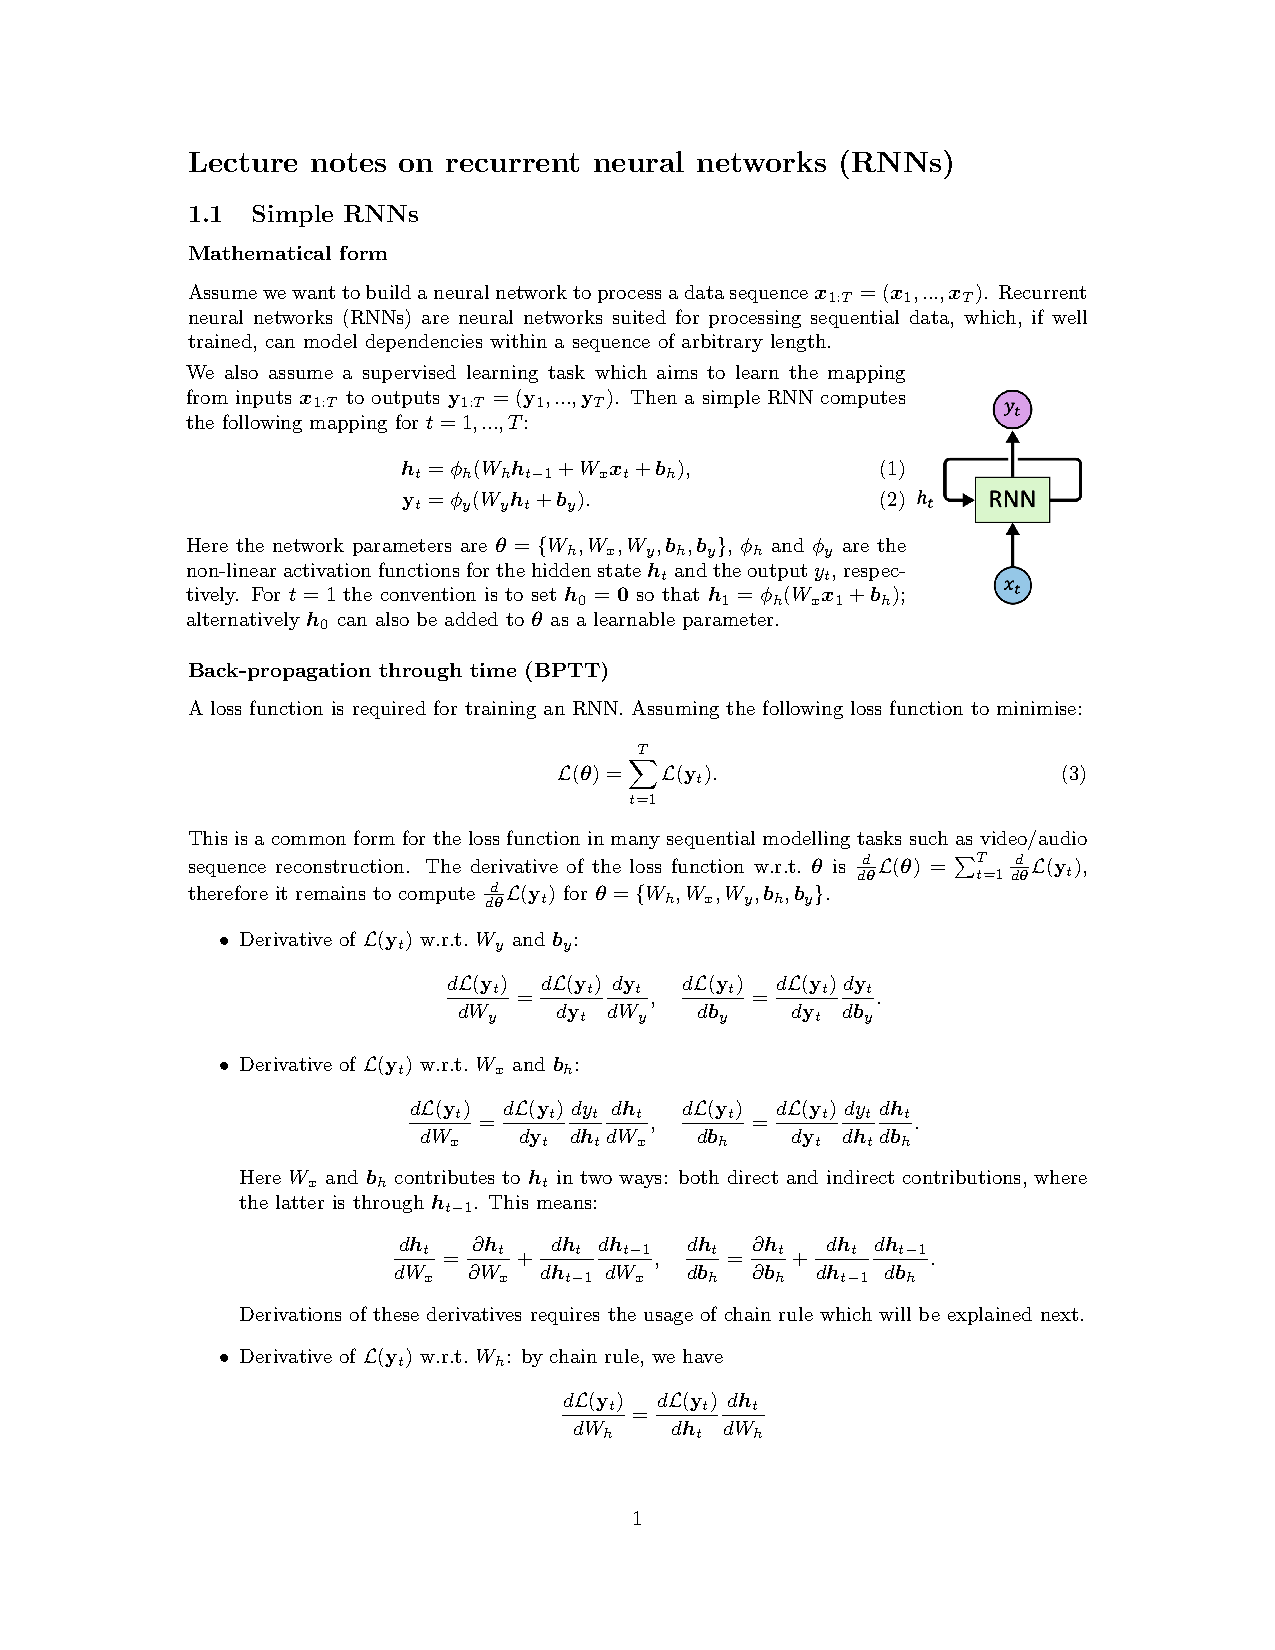
\includegraphics[page=1, trim=3cm 17cm 3cm 4.7cm, clip=true, width=.95\linewidth]{N11_RNN.pdf}}
\end{figure}

\subsection{Training RNNs}

\subsubsection{Back-propagation through time (BPTT)}

% \begin{figure}[H]
%     \centering
%     \fbox{\includegraphics[page=10, trim=1cm 2.7cm 8cm 4.5cm, clip=true, width=.95\linewidth]{L11-14_rnns.pdf}}
%     \caption*{Training the neural network}
% \end{figure}

\begin{figure}[H]
    \centering
    \fbox{\includegraphics[page=2, trim=3cm 19.5cm 3cm 2.5cm, clip=true, width=.95\linewidth]{N11_RNN.pdf}}
\end{figure}

We want to minimise the loss of $\mathcal L(\vec\theta)=L_{total}(\vec \theta)=\sum^T_{t=1}L(y_t)$ using gradient descent. This means we need to compute the gradient of the loss with respect to the parameters of the model.  

\begin{figure}[H]
    \centering
    \fbox{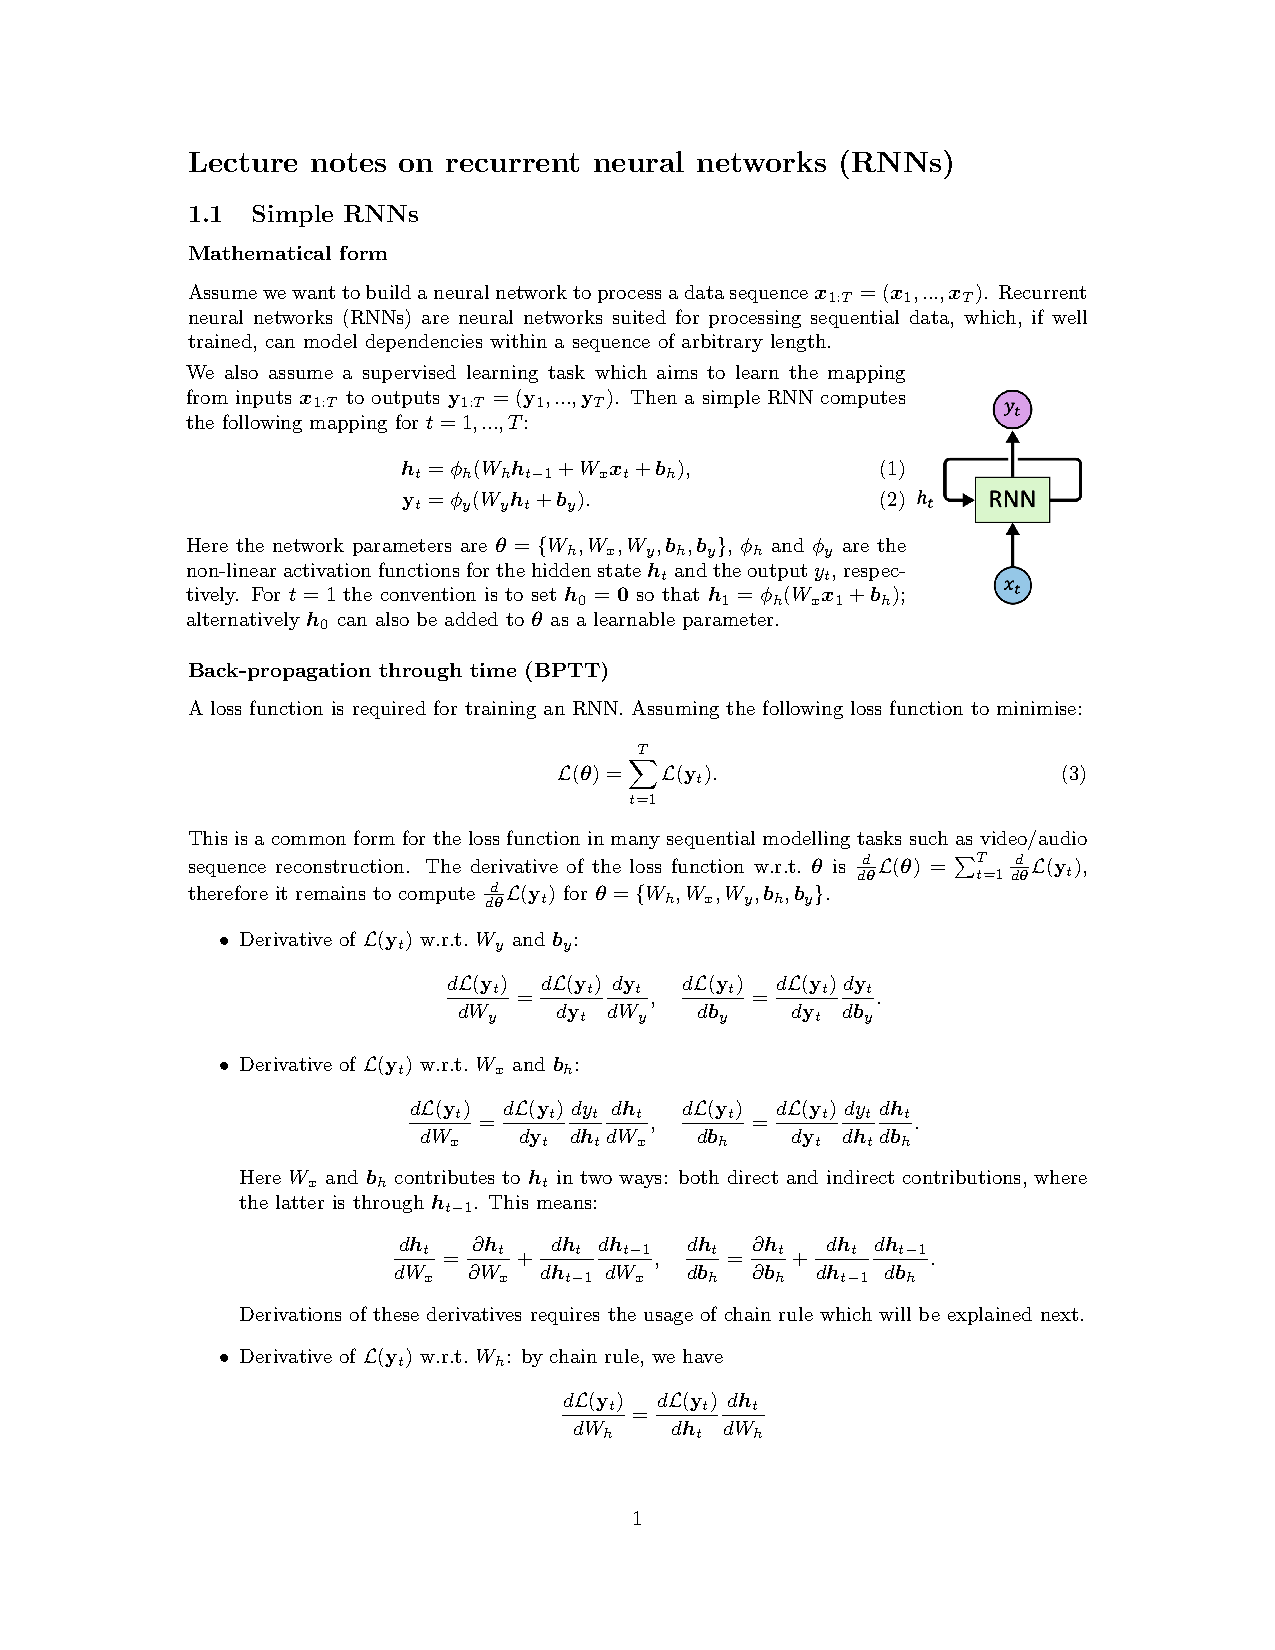
\includegraphics[page=1, trim=3cm 12.5cm 3cm 11.6cm, clip=true, width=.95\linewidth]{N11_RNN.pdf}}
\end{figure}

\begin{figure}[H]
    \centering
    \fbox{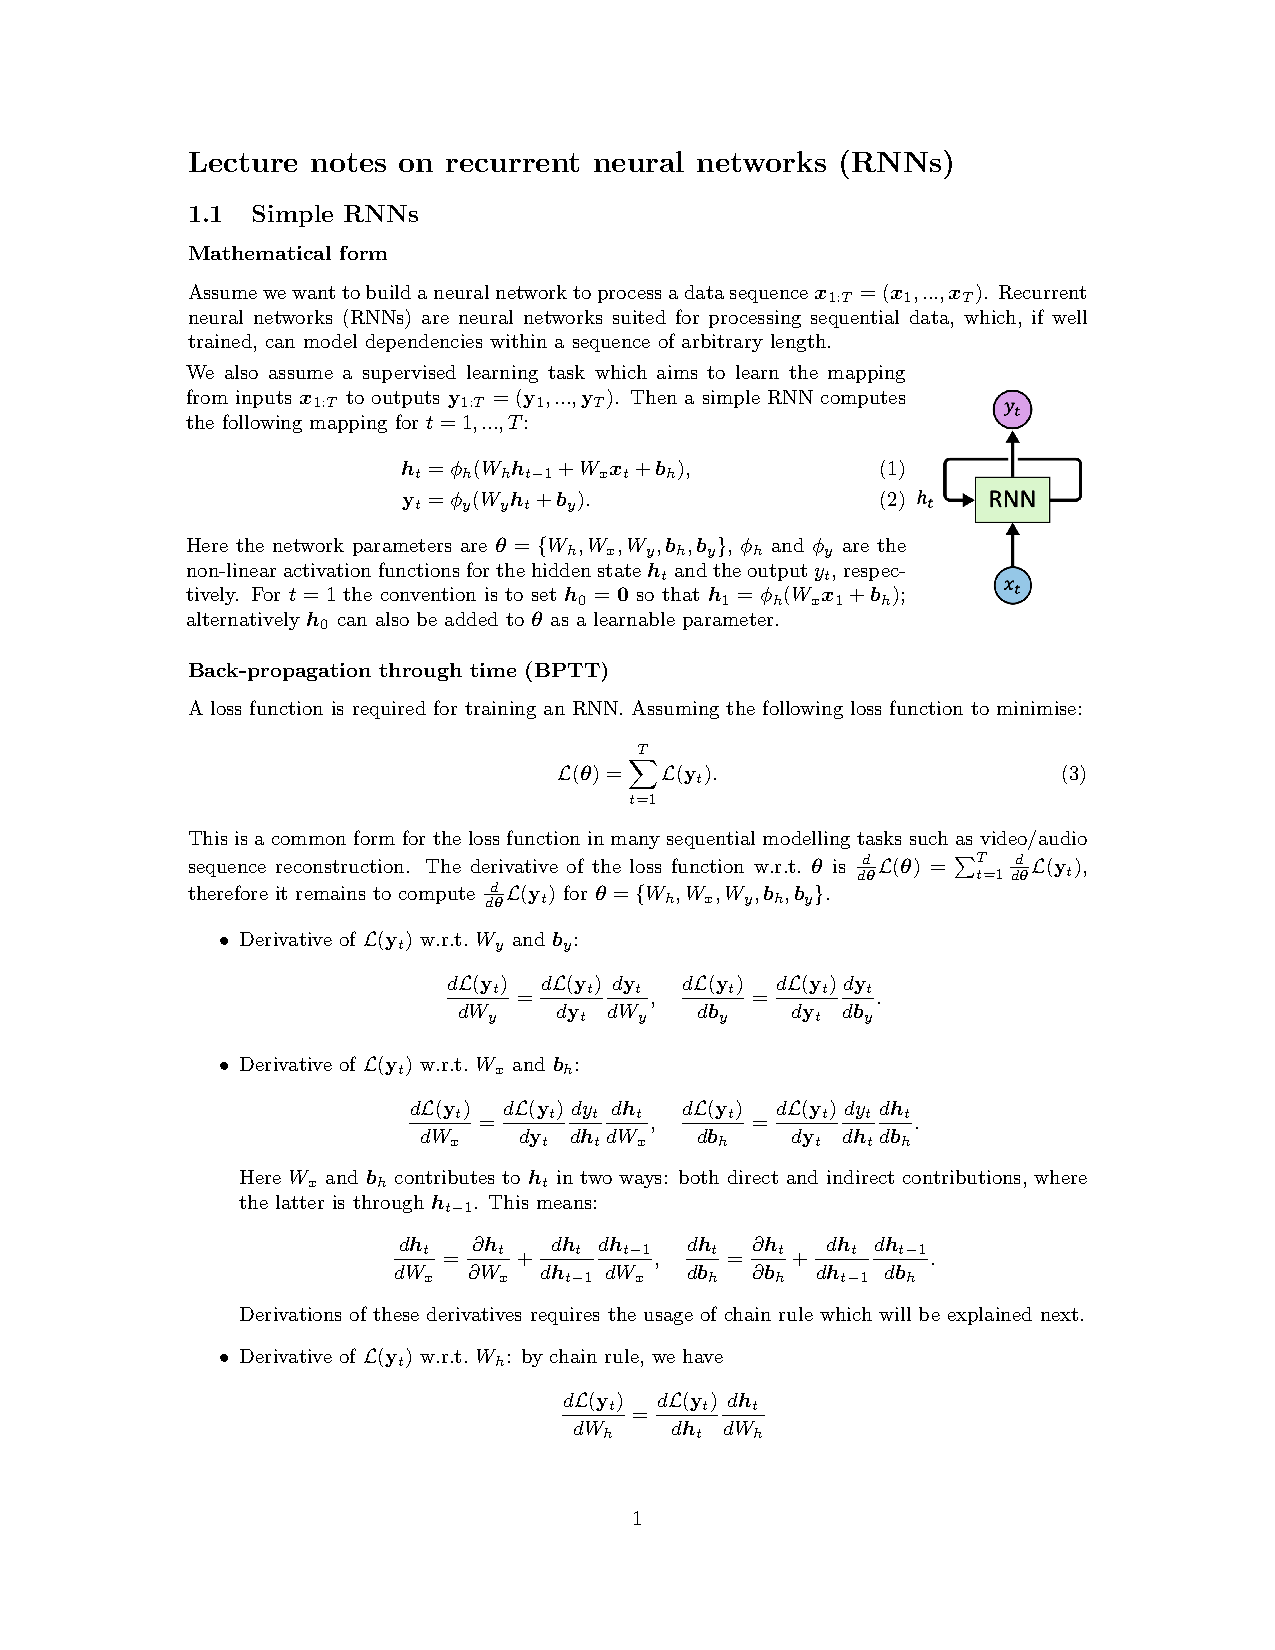
\includegraphics[page=1, trim=3cm 3.5cm 3cm 15.5cm, clip=true, width=.95\linewidth]{N11_RNN.pdf}}
    \fbox{\includegraphics[page=2, trim=3cm 9cm 3cm 8.8cm, clip=true, width=.95\linewidth]{N11_RNN.pdf}}
\end{figure}

\subsubsection{Gradient vanishing/explosion issues}

Depending on the weight matrix and the activation function the product of the partial graident can vanish or explode as the number of time steps increases.

\begin{figure}[H]
    \centering
    \fbox{\includegraphics[page=2, trim=3cm 3cm 3cm 20.3cm, clip=true, width=.95\linewidth]{N11_RNN.pdf}}
    \caption*{Here, the circled dot operator is typically used to represent element-wise multiplication}
\end{figure}

\begin{figure}[H]
    \centering
    \fbox{\includegraphics[page=3, trim=3cm 15.6cm 3cm 2.5cm, clip=true, width=.95\linewidth]{N11_RNN.pdf}}
\end{figure}

Therefore, long term dependencies are getting harder to learn. With vanishing gradient, Since the gradient for $W_h$ is the sum of back-prop gradient with different window length, this gradient will be dominated especially when $t >> \tau$; the learning signal will be dominated by the short term dependencies.

\begin{figure}[H]
    \centering
    \fbox{\includegraphics[page=17, trim=3cm 3cm 4cm 11cm, clip=true, width=.95\linewidth]{L11-14_rnns.pdf}}
    % \caption*{}
\end{figure}

Tricks for how to fix the gradient vanishing or explosion issue are detailed in the Appendix~\ref{app:tricks-gradient-v/e}.

\section{Long Short-Term Memory (LSTM)}

\subsection{Forward Pass}

\begin{figure}[H]
    \centering
    \fbox{\includegraphics[page=18, trim=6cm 5.5cm 6cm 4.5cm, clip=true, width=.95\linewidth]{L11-14_rnns.pdf}}
    \caption*{Addresses the problem of gradient descent problem. They perform better at learning long-term dependencies than simple RNNs}
\end{figure}

The Long Short-term Memory was proposed with the motivation of adderssing the graident vanishing/explosion problem. It introduces memory cell states and gates to control the error flows, in detail the computation goes as follows (with $\sigma(\cdot)$ as sigmoid funciton):

\begin{figure}[H]
    \centering
    \fbox{\includegraphics[page=4, trim=3cm 19.3cm 3cm 3.3cm, clip=true, width=.95\linewidth]{N11_RNN.pdf}}
    \caption*{Here, commas (e.g.) $[h_{t-1},x_t]$ mean concatenations}
\end{figure}

\begin{figure}[H]
    \centering
    \subfigure
        [Forget gate: used to control the cell state update. It depends on the previous hidden state and current input. This is a one layer network with sigmoid activation function. Equation (7) above.]
        {
            \fbox{\includegraphics[page=19, trim=3.3cm 6.5cm 21.5cm 6.5cm, clip=true, width=.3\linewidth]{L11-14_rnns.pdf}}
    }
    \subfigure
        [The second step is to propose a cnadidate update value $\tilde{c}_t$ to the cell state. In this case an input gate is also computed to form the cell state value as well. Equations (8) and (10) above.]
        {
            \fbox{\includegraphics[page=20, trim=3.3cm 6.5cm 21.5cm 6.5cm, clip=true, width=.3\linewidth]{L11-14_rnns.pdf}}
    }
    \subfigure
        [Cell state update. $f_t$ controls the maintenance of the previous cell states. Similarly, the input gate controlls whether the candidate update will be accepted or not. Equation (11) above.]
        {
            \fbox{\includegraphics[page=21, trim=3.3cm 6.5cm 21.5cm 6.5cm, clip=true, width=.3\linewidth]{L11-14_rnns.pdf}}
    }
\end{figure}

\begin{figure}[H]
    \centering
    \subfigure
        [Finally, compute the updates for the hidden states $h_t$. Here $h_t$ is used to output a cell state $c_t$. But here, an output gate is also being used. THis means sometimes the hidden state will be 0 given the output gate values. Equations (9) and (12) above.]
        {
            \fbox{\includegraphics[page=22, trim=3.3cm 6.5cm 21.5cm 6.5cm, clip=true, width=.3\linewidth]{L11-14_rnns.pdf}}
    }
    \caption*{The Prediction of $y_t$ can proceed in a simlar way as in simple RNNS: $y_t = \Phi_y(W_yh_t + b_y)$ by transforming the hidden state $h_t$ with one neural network layer.}
\end{figure}

\subsection{Backwards Pass}

In this case, the recurrent state we care about is the cell state $c_t$. Back-prop thorugh time applies to computing the graident with respect to $W_c$ the weight matrix for computing the candidate cell state. 


\subsubsection{\color{red}{*Gradient computation}}

\begin{figure}[H]
    \centering
    \fbox{\includegraphics[page=23, trim=2.5cm 7cm 15cm 7.1cm, clip=true, width=.7\linewidth]{L11-14_rnns.pdf}}
    \caption*{``To give an idea of how this gradient is derrived, we can look at the recurrent update equation for the cell state $c_t$. Here, $c_t$ depends on $c_{t-1}$ as shown in the red box. However, there are also indirect paths via $f_t \wedge i_t \wedge c_t$ because they all depend of $h_{t-1}$ which depends on $c_{t-1}$. This gives us an idea of how to compute the total gradient.''}
\end{figure}

\begin{figure}[H]
    \centering
    \fbox{\includegraphics[page=4, trim=3cm 3cm 3cm 9.8cm, clip=true, width=.9\linewidth]{N11_RNN.pdf}}
\end{figure}

\begin{figure}[H]
    \centering
    \fbox{\includegraphics[page=5, trim=3cm 17cm 3cm 2.5cm, clip=true, width=.9\linewidth]{N11_RNN.pdf}}
\end{figure}

\subsection{How LSTMs alleviate training difficulties of RNNs}

\begin{figure}[H]
    \centering
    \fbox{\includegraphics[page=24, trim=2.4cm 1.1cm 0.5cm 4.2cm, clip=true, width=.95\linewidth]{L11-14_rnns.pdf}}
    \caption*{The usage of forget gates is useful for gradient explosion problems, becuase the network can learn a forget gate value of 0. Similarly, the product of gradients after expansion contains terms like product of $f_t$ terms times other terms. If the forget gates are open, then this term becomes the gradient of $c_{\tau+1}$ with resepect ot $h_\tau$. If $\tau$ is small and $i$ is big, then errors can also be back-propogated and doesn't vanish. This is useful for learning long-term dependencies.}
\end{figure}

\subsection{Alternatives | Gated Recurrent Unit (GRU)}

\begin{minipage}[l]{.4\linewidth}
    \begin{figure}[H]
        \centering
        \fbox{\includegraphics[page=25, trim=3cm 6.5cm 22cm 6.3cm, clip=true, width=0.95\linewidth]{L11-14_rnns.pdf}}
    \end{figure}
\end{minipage}\hfill
\begin{minipage}[r]{.55\linewidth}
    Simplified versions of the LSTM have been proposed. Compared to LSTMs, GRU only uses switching gates $z_t$ and reset gates $r_t$. you can still see that GRU still implements gating mechanisms to control the updates fo rthe recurrent states.
\end{minipage}

\begin{figure}[H]
    \centering
    \fbox{\includegraphics[page=5, trim=3cm 10.5cm 3cm 12cm, clip=true, width=.95\linewidth]{N11_RNN.pdf}}
\end{figure}

\subsubsection{LSTM vs GRU}

\begin{itemize}
    \item Other gated RNN variants exists, but LSTM and GRU are the most widely-used
    \item GRU is quicker to compute and has fewer parameters
    \item No conclusive evidence for LSTM $>$ GRU or vice versa
    \item LSTM is a good default choice (especially if your data has particularly long dependencies, or you have lots of training data)
    \item Switch to GRU if you want more efficient compute \& less overfitting
\end{itemize}

\subsection{Stacking LSTMs}

\begin{figure}[H]
    \centering
    \fbox{\includegraphics[page=27, trim=2cm 4cm 2cm 5.3cm, clip=true, width=0.95\linewidth]{L11-14_rnns.pdf}}
\end{figure}

\subsection{Bidirectional LSTMs}

\begin{figure}[H]
    \centering
    \fbox{\includegraphics[page=28, trim=2cm 4cm 2cm 5.3cm, clip=true, width=0.95\linewidth]{L11-14_rnns.pdf}}
    \caption*{Has shown to improve performance}
\end{figure}

\section{Sequence-to-sequence models}

\begin{figure}[H]
    \centering
    \fbox{\includegraphics[page=5, trim=3cm 3cm 3cm 18.5cm, clip=true, width=.95\linewidth]{N11_RNN.pdf}}
    \caption*{Here, the auto-regression model means that the output $y$ sequence is generated in a sequential way, and the current location $y_l$ depends on the y values at all the previous steps.}
\end{figure}

\begin{figure}[H]
    \centering
    \fbox{\includegraphics[page=32, trim=3.2cm 2.5cm 11.5cm 4.5cm, clip=true, width=.7\linewidth]{L11-14_rnns.pdf}}
    % \caption*{The ingredients in the sequence to sequence model.}
\end{figure}

First, we need a sequnce encoder to summarise the information presented in the X sequence. We know that X sequence can have different lenghts, but RNNs can handle this situation. Firstly, we map words ino word embeddings before we feed them into neural networks. Here, one-hot encoding is inefficient (sparse and many demensions). Then, use an LSTM or Stacked LSTM to process each of the word embedding vectors. We don't generate outputs at each time-step $t$ here, instead at the end we use the hidden state $h_t$ to fully describe the input seqeunce $X$. Note, we also need to have an end of sentence token so it may terminates (good cuz not fixed length).

\begin{figure}[H]
    \centering
    \fbox{\includegraphics[page=34, trim=3.2cm 2.5cm 3.2cm 4.5cm, clip=true, width=.95\linewidth]{L11-14_rnns.pdf}}
    % \caption*{The ingredients in the sequence to sequence model.}
\end{figure}

Now, given the vector representation $v$, how do we generate the output sequences? Since $v$ is related closely to the last LSTM state $h_t$ in a sequence to sequnce model, it can be used to produce the probability of the first word $y_1$ in the $y$ output sequence. Then the first word will be sampled from this probability vector.

Given $y_1$ the seqeunce decoder proceeds to predict the next word in the $y$ sequence. The sequence decoder is also an LSTM. At each time step for prediction, the decoder LSTM takes in the word embeddings of the predicted word in the last step then runs the LSTM equation to update the internal state. Now, the decoder LSTM will predict the probabilitiy vector for the output word $y_l$ at each time step. The representation vector $v$ of the input sentence is used to initialise the hidden and cell states of the decoder LSTM. It will run until the end-of-sentence token.

\begin{figure}[H]
    \centering
    \fbox{\includegraphics[page=6, trim=3cm 15.6cm 3cm 10.2cm, clip=true, width=.95\linewidth]{N11_RNN.pdf}}
\end{figure}

\subsection{Sequence decoder inputs during training/testing}

\begin{figure}[H]
    \centering
    \fbox{\includegraphics[page=6, trim=3cm 18.5cm 3cm 2.5cm, clip=true, width=.95\linewidth]{N11_RNN.pdf}}
\end{figure}

In training, since maximum likelihood estimation of the network parameters require calculating the conditional probability distribution from the $x,y$ data piars. This means that the decoder needs to use the input labels $y$ rather than using the predicted $y$ predicted in the previous steps. The probability vectors produced by the decoders in training are only used to compute the training objective (cross-entropy loss) to train the network during back-prob. But during the test, we should use the previous predicted words as the inputs at the current steps.

\begin{figure}[H]
    \centering
    \fbox{\includegraphics[page=6, trim=3cm 3.8cm 3cm 12.3cm, clip=true, width=.95\linewidth]{N11_RNN.pdf}}
\end{figure}

This sort of encoding decoding idea cna be extended to other applications, such as image captioning. 

\begin{figure}[H]
    \centering
    \fbox{\includegraphics[page=36, trim=3.2cm 2.5cm 1.8cm 4.5cm, clip=true, width=.95\linewidth]{L11-14_rnns.pdf}}
    \caption*{The goal is to decribe an image with a sentence. A popular approach is to ENCODE a feature representation of image $x$ and use this to intialise the LSTM and run the decoder LSTM to produce a sentence.}
\end{figure}

\subsection{\color{red}{*Generative models for sequences} | Sequence VAE}

To generate sequential data dsuch as video, text and audio, one needs to build a generativemodel $p_\theta(x_{1:T})$ and train it with e.g. (approximate) maximum likelihood. In the following we discuss tow types of latent variable models that are often used in sequence generation tasks.

\begin{figure}[H]
    \centering
    \fbox{\includegraphics[page=7, trim=3cm 18.1cm 3cm 5.6cm, clip=true, width=.9\linewidth]{N11_RNN.pdf}}
    \caption*{Contains the training objective function. Here, $\log p_\theta(x_{1:T}|z) = \sum^T_{t=1}\log p_\theta(x_t | x_{<t}, z)$
    
    We may also use a $\beta$ coefficient infront of the $KL$ term, to control the deregularisation effect. It has shown to be a quite important to achieve a good fit to data, and high quality generation results.}
\end{figure}

\begin{figure}[H]
    \centering
    \fbox{\includegraphics[page=38, trim=3.2cm 2.3cm 1.8cm 6.2cm, clip=true, width=.9\linewidth]{L11-14_rnns.pdf}}
    \caption*{The solution is similar to the image captioning task. We can build an auto-regressive model for the conditional distribution of $x$ 1 to t given $z$. This auto regressive model is parameterised by an LSTM, which takes in the previous $x$ words to produce the current output $x_t$. The latent varibale $z$ can be used to initialise the decoder.
    
    We can use a VAE appraoch to train these sequence gerneation models. We need to build an encoder (use LSTM) but here, at the end, the encoder needs to produce distirbutional parmaeters of the q distribution like mean and variance. This is similar to the image in VEA case, except now the input and output are sequences from a static image.}
\end{figure}

\begin{figure}[H]
    \centering
    \fbox{\includegraphics[page=7, trim=3cm 13.6cm 3cm 10.3cm, clip=true, width=.9\linewidth]{N11_RNN.pdf}}
\end{figure}

\subsection{State-space models}

\begin{figure}[H]
    \centering
    \fbox{\includegraphics[page=40, trim=3cm 1.8cm 3cm 7.9cm, clip=true, width=.9\linewidth]{L11-14_rnns.pdf}}
    \caption*{In a state-space model, it has a stochastic dynamic model for the latent state. In other words, the latent varibale $z$ is split, with each $z_t$ associated with each state time step, depending on previous latent states.
    
    It also contains an emission model, where the assumption is that the generation of the current $x_t$ depends on the $z_t$ only.}
\end{figure}


\begin{figure}[H]
    \centering
    \fbox{\includegraphics[page=7, trim=3cm 3cm 3cm 15.2cm, clip=true, width=.95\linewidth]{N11_RNN.pdf}}
\end{figure}

\subsubsection{Hidden Markov Model}

\begin{figure}[H]
    \centering
    \fbox{\includegraphics[page=41, trim=3cm 6cm 3cm 7cm, clip=true, width=.9\linewidth]{L11-14_rnns.pdf}}
    \caption*{This model assume a stochastic linear dynamic model fro the latent space, meaning that the current latent state $x_t$ is computed by a linear transition of the previous state $z_{t-1}$ plus some gaussian noise. 
    
    Also, it has a linear Guasisnan emission model. So that the observation at time T is also a linear transfomration of the correlated state $z_t$ plus gaussian noise.
    
    This is linear and stochastic; add a non-linearity model to the transition model of $z$ and make the dynamic model a simple and stochastic RNN. Yet, this is difficult to train (see seciton regarding RNNs)}
\end{figure}

\begin{figure}[H]
    \centering
    \fbox{\includegraphics[page=43, trim=3cm 2.5cm 1.5cm 6.7cm, clip=true, width=.9\linewidth]{L11-14_rnns.pdf}}
    \caption*{
        A typical solution for a paramaeterising the stochastic dyanmic model with LSTMs. The idea is to treat the previous latent space $z_{t-1}$ as input to the LSTM at time $t$ and ask the LSTM to produce the distirbution parmaeters (mean and variance) for the current latent state $z_t$. 
        
        Now the dynamic model is a combination of deterministic and stochastic models. We can make it non-linear. See slide.

        The joint distribution contains the conditional distributions of the latent dynamic model and the emission model. For the emission model it is similar to writing the conditional distribution int eh iamge generative model case.

        \color{red}{TODO WTF IS GOING ON??}
    }
\end{figure}

\subsubsection{Training}

\begin{figure}[H]
    \centering
    \fbox{\includegraphics[page=44, trim=3cm 2cm .8cm 6.2cm, clip=true, width=.95\linewidth]{L11-14_rnns.pdf}}
    \caption*{
        \color{red} TODO WTF IS GOING ON!!!!
    }
\end{figure}

\begin{figure}[H]
    \centering
    \fbox{\includegraphics[page=8, trim=3cm 12.5cm 3cm 2.5cm, clip=true, width=.95\linewidth]{N11_RNN.pdf}}
\end{figure}

\section{Attention \& Transformers}

\subsection{Motivation}

\begin{figure}[H]
    \centering
    \fbox{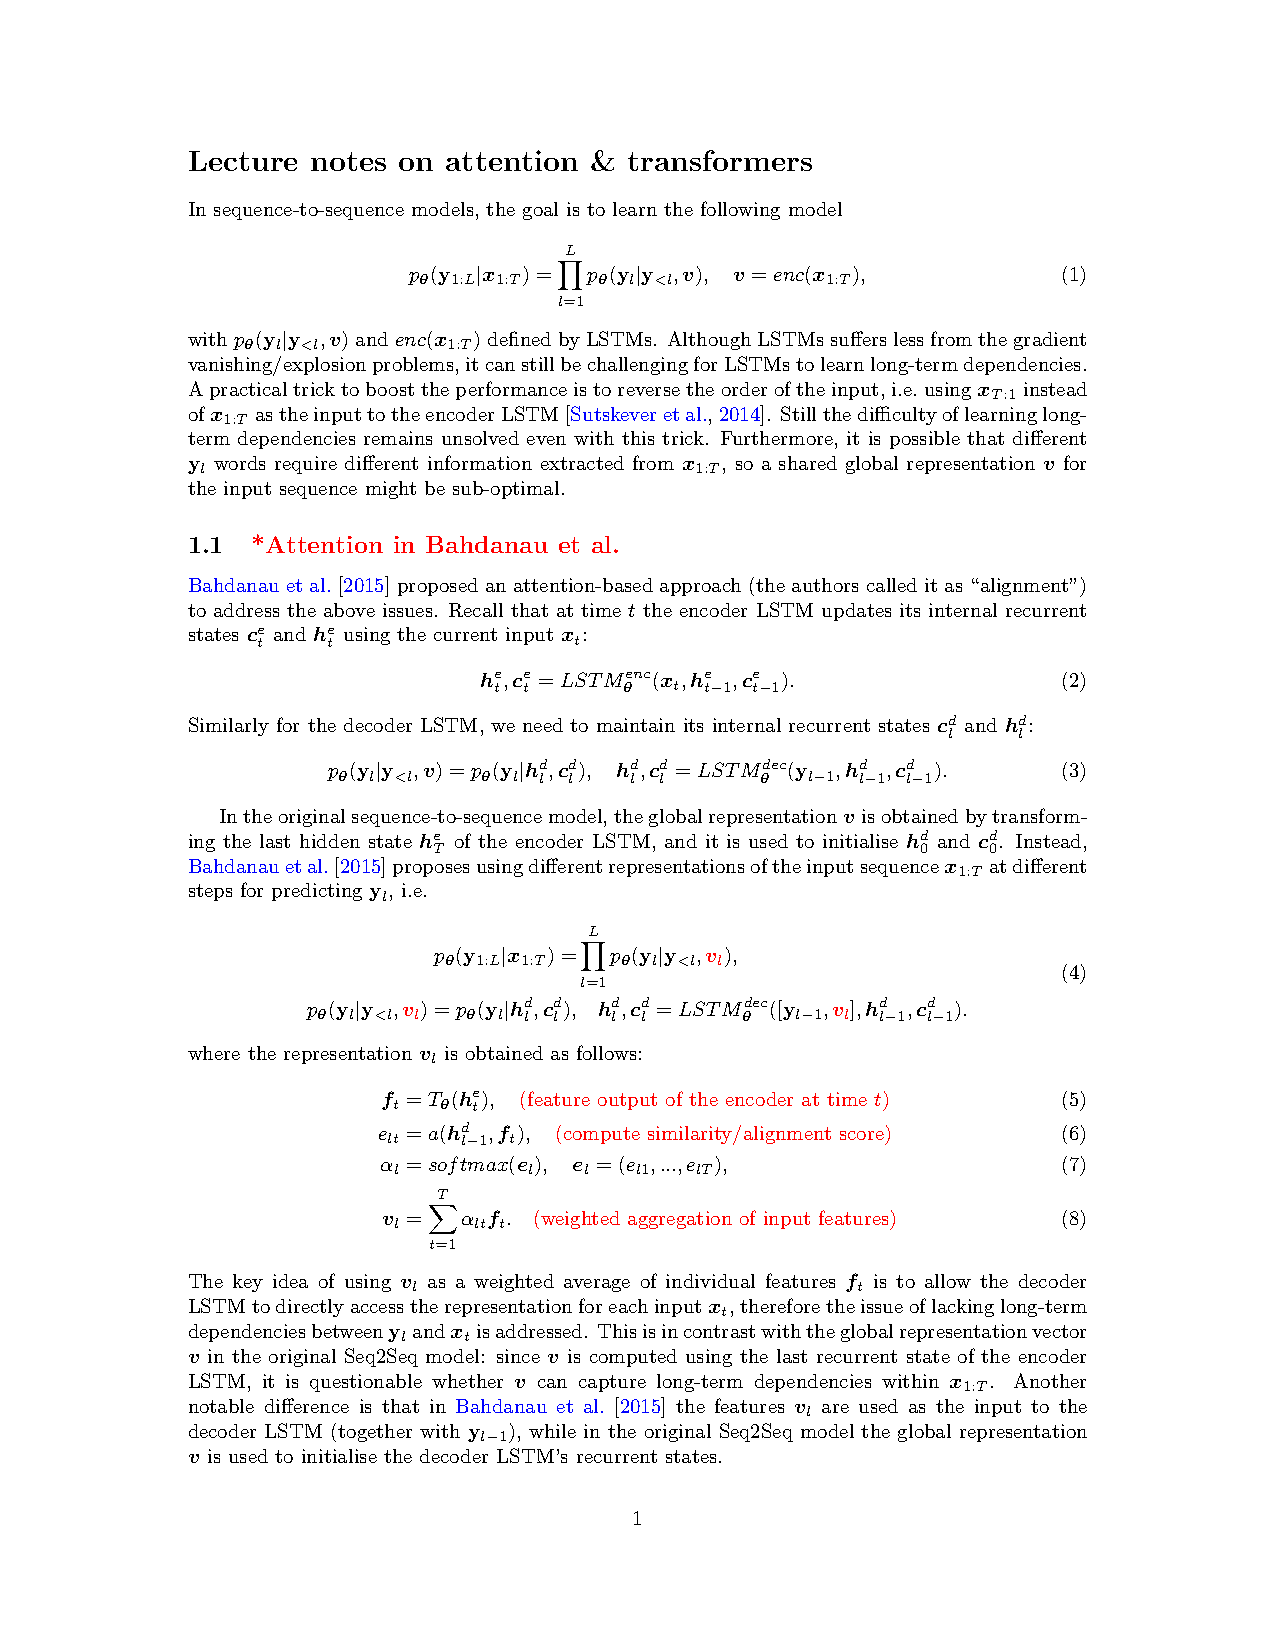
\includegraphics[page=1, trim=3cm 19.5cm 3cm 3.3cm, clip=true, width=.95\linewidth]{N13_attention.pdf}}
    \caption*{
        People have found that as the sentence length has increased, the quality of the sentence decreases. This is a problem, since a lot of sequenced data is very long naturally.
    }
\end{figure}

\subsection{NMT model}

\begin{figure}[H]
    \centering
    \fbox{\includegraphics[page=50, trim=1cm 1.3cm 2cm 4cm, clip=true, width=.95\linewidth]{L11-14_rnns.pdf}}
\end{figure}

\begin{enumerate}
    \item The first attempt is to improve the sequnce to sequnce model with attention. In SeS the global representation vector v is used to represent the entire input seqeunce for all y. This means it need to capture as much informatino as possible, yet, it comes from the last state in the LSTM | this means that there may be problems of learning long-term dependencies.
    \item Bahdanau proposed to use different feature vectors at different decoding steps to represent the input sequence. The idae: decoding words at different states, the context can be different. Therefore, don't use only the last state - we ask the encoder to produce a feature output $f$ at each time step, and compute a weighted sum of those features to obtain a feature represnetiaton of the input sequence.
    \item $\alpha$ is different at each decoding step. This depends on the alignment/similarity between the feature $f_t$ and the representatino of the current decoding step.
\end{enumerate}

\begin{figure}[H]
    \centering
    \fbox{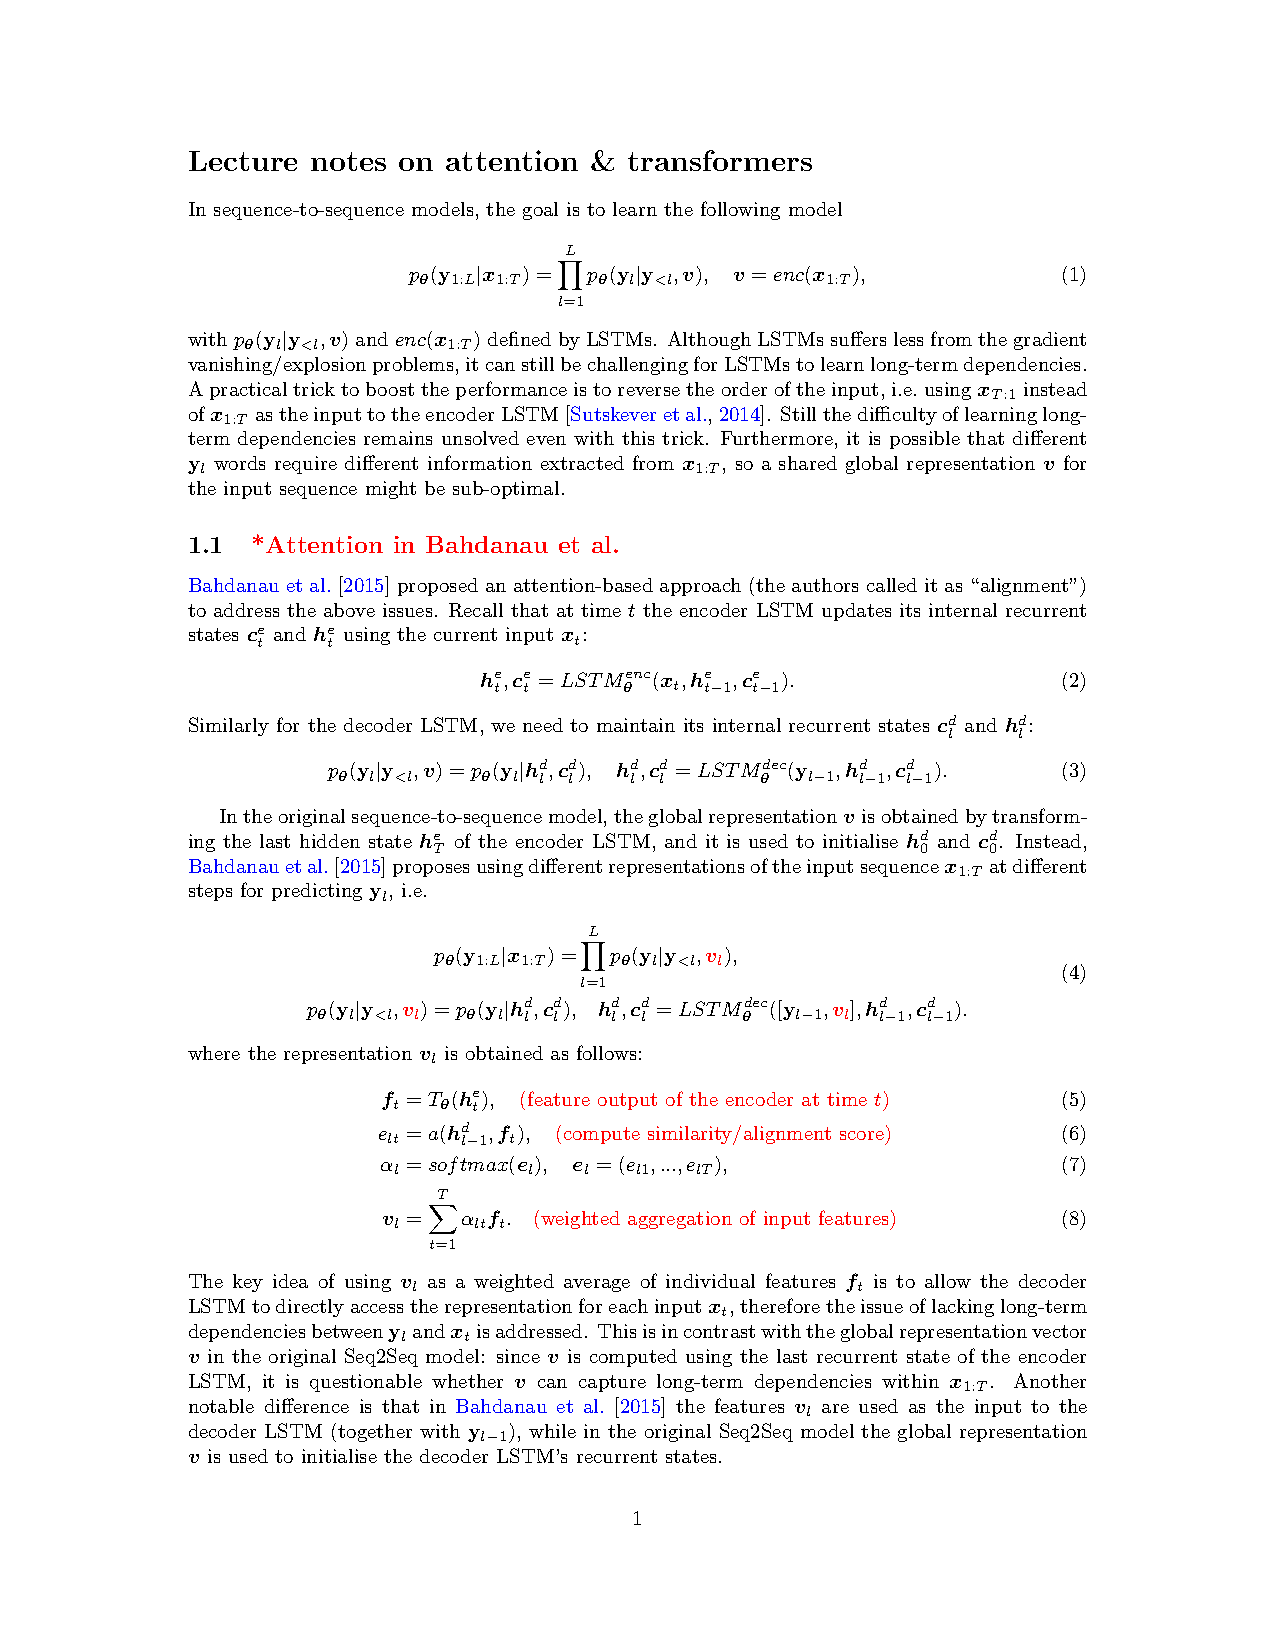
\includegraphics[page=1, trim=3cm 3cm 3cm 9.6cm, clip=true, width=.95\linewidth]{N13_attention.pdf}}
\end{figure}

\begin{figure}[H]
    \centering
    \fbox{\includegraphics[page=2, trim=3cm 23.2cm 3cm 2.5cm, clip=true, width=.95\linewidth]{N13_attention.pdf}}
\end{figure}

\subsection{Attention in Transformers | Single-head attention}

\begin{figure}[H]
    \centering
    \fbox{\includegraphics[page=51, trim=2cm 2.7cm 1cm 4cm, clip=true, width=.95\linewidth]{L11-14_rnns.pdf}}
\end{figure}

\begin{figure}[H]
    \centering
    \fbox{\includegraphics[page=2, trim=3cm 5.5cm 3cm 6.5cm, clip=true, width=.95\linewidth]{N13_attention.pdf}}
\end{figure}

\subsubsection{Hard-attention}

\begin{figure}[H]
    \centering
    \fbox{\includegraphics[page=52, trim=2cm 2cm 4cm 5cm, clip=true, width=.95\linewidth]{L11-14_rnns.pdf}}
\end{figure}

\subsubsection{Soft-attention}

\begin{figure}[H]
    \centering
    \fbox{\includegraphics[page=53, trim=2cm 2.6cm 4cm 5cm, clip=true, width=.95\linewidth]{L11-14_rnns.pdf}}
\end{figure}

\subsubsection{Msked-attention}

\begin{figure}[H]
    \centering
    \fbox{\includegraphics[page=54, trim=2cm 3cm 4cm 5cm, clip=true, width=.95\linewidth]{L11-14_rnns.pdf}}
\end{figure}

\subsubsection{Complexity analysis}

\begin{figure}[H]
    \centering
    \fbox{\includegraphics[page=55, trim=2cm 4cm 4cm 5cm, clip=true, width=.95\linewidth]{L11-14_rnns.pdf}}
\end{figure}

\begin{figure}[H]
    \centering
    \subfigure{
        \fbox{\includegraphics[page=2, trim=3cm 3cm 3cm 23.5cm, clip=true, width=.95\linewidth]{N13_attention.pdf}}    
    }
    \subfigure{
        \fbox{\includegraphics[page=3, trim=3cm 23.2cm 3cm 2.5cm, clip=true, width=.95\linewidth]{N13_attention.pdf}}   
    }
\end{figure}

\subsection{Attention in Transformers | Multi-head attention}

\begin{figure}[H]
    \centering
    \fbox{\includegraphics[page=56, trim=2cm 3cm 1cm 4cm, clip=true, width=.95\linewidth]{L11-14_rnns.pdf}}
\end{figure}

\begin{figure}[H]
    \centering
    \fbox{\includegraphics[page=57, trim=2cm 2.7cm 1cm 4cm, clip=true, width=.95\linewidth]{L11-14_rnns.pdf}}
\end{figure}

\begin{figure}[H]
    \centering
    \fbox{\includegraphics[page=3, trim=3cm 10.5cm 3cm 5.8cm, clip=true, width=.95\linewidth]{N13_attention.pdf}}
\end{figure}

\subsection{Transformer Architecture}

\begin{figure}[H]
    \centering
    \fbox{\includegraphics[page=3, trim=3cm 8.5cm 3cm 18.5cm, clip=true, width=.95\linewidth]{N13_attention.pdf}}
\end{figure}

\begin{figure}[H]
    \centering
    \fbox{\includegraphics[page=4, trim=5.5cm 17cm 5.5cm 2.5cm, clip=true, width=.95\linewidth]{N13_attention.pdf}}
\end{figure}

We first want to use the Attention based encoder to extract features for input sequences $x_{1:T}$. Then we will follow the autoregressive decoding process again to produce the output sequence, but different from the Sequence to sequnce model; now the decoder is also an attention based network,rather than LSTM. 

\begin{equation}
    p_\theta(y_{1:L}|x_{1:T}) = \prod^L_{l=1}p_\theta(y_l|y_{<l},z_{1:T})
\end{equation}

The first step in the encoding process is to gether input embeddings for the input sequence. In an NLP setting, this is the word embeddings. BEfore we feed in the input representationso, we append the input embedding with a position encoding. {\color{red}TODO}

\begin{figure}[H]
    \centering
    \fbox{\includegraphics[page=59, trim=3cm 4cm 3cm 6cm, clip=true, width=.95\linewidth]{L11-14_rnns.pdf}}
    % \caption*{\color{red}TODO}
\end{figure}

\begin{figure}[H]
    \centering
    \fbox{\includegraphics[page=60, trim=1.7cm 1.3cm 1.7cm 3.4cm, clip=true, width=.95\linewidth]{L11-14_rnns.pdf}}
    % \caption*{\color{red}TODO}
\end{figure}

\begin{figure}[H]
    \centering
    \fbox{\includegraphics[page=61, trim=1.7cm 1.3cm 1.7cm 3.4cm, clip=true, width=.95\linewidth]{L11-14_rnns.pdf}}
    % \caption*{\color{red}TODO}
\end{figure}

\begin{figure}[H]
    \centering
    \fbox{\includegraphics[page=62, trim=1.7cm 1.3cm 1.7cm 3.4cm, clip=true, width=.95\linewidth]{L11-14_rnns.pdf}}
    % \caption*{\color{red}TODO}
\end{figure}

\begin{figure}[H]
    \centering
    \fbox{\includegraphics[page=63, trim=1.7cm 1.3cm 1.7cm 3.4cm, clip=true, width=.95\linewidth]{L11-14_rnns.pdf}}
    % \caption*{\color{red}TODO}
\end{figure}

\begin{figure}[H]
    \centering
    \fbox{\includegraphics[page=64, trim=1.7cm 1.3cm 1.7cm 3.4cm, clip=true, width=.95\linewidth]{L11-14_rnns.pdf}}
    % \caption*{\color{red}TODO}
\end{figure}

\begin{figure}[H]
    \centering
    \fbox{\includegraphics[page=65, trim=1.7cm 1.3cm 1.7cm 3.4cm, clip=true, width=.95\linewidth]{L11-14_rnns.pdf}}
    % \caption*{\color{red}TODO}
\end{figure}

\section{Advances and Applications}

\subsection{Attention Applications}

\begin{figure}[H]
    \centering
    \fbox{\includegraphics[page=67, trim=1.7cm 1.3cm 1.7cm 3.6cm, clip=true, width=.95\linewidth]{L11-14_rnns.pdf}}
    \caption*{pen position and pen position wasn't aligned | author developed an RNN}
\end{figure}

\begin{figure}[H]
    \centering
    \fbox{\includegraphics[page=68, trim=1.7cm 4cm 1.7cm 3.6cm, clip=true, width=.95\linewidth]{L11-14_rnns.pdf}}
    \caption{}
\end{figure}

\begin{figure}[H]
    \centering
    \fbox{\includegraphics[page=69, trim=1.7cm 1.3cm 1.7cm 4cm, clip=true, width=.95\linewidth]{L11-14_rnns.pdf}}
    \caption{before we use CNNs to extract features from images, and then use RNNs to generate captions. Now, since the CNN captures spatial location we can treat these features as an input sequence indexed by the spatial locaiton. Then apply Seq2Seq.}
\end{figure}

\subsection{Transformer in NLP}

\begin{figure}[H]
    \centering
    \fbox{\includegraphics[page=70, trim=1.7cm 1.3cm 1.7cm 3.6cm, clip=true, width=.95\linewidth]{L11-14_rnns.pdf}}
    \caption{Attention based. We mask and pre-train.}
\end{figure}

\begin{figure}[H]
    \centering
    \fbox{\includegraphics[page=71, trim=1.7cm 1.3cm 1.7cm 3.6cm, clip=true, width=.95\linewidth]{L11-14_rnns.pdf}}
    \caption{}
\end{figure}

\subsection{Multi-head Attention in other applications}

\begin{figure}[H]
    \centering
    \fbox{\includegraphics[page=72, trim=1.7cm 1.3cm 1.7cm 3.6cm, clip=true, width=.95\linewidth]{L11-14_rnns.pdf}}
    \caption{Trnasformers can be applied to any domain where data comes in sets}
\end{figure}

\begin{figure}[H]
    \centering
    \fbox{\includegraphics[page=73, trim=1.7cm 1.3cm 1.7cm 3.6cm, clip=true, width=.95\linewidth]{L11-14_rnns.pdf}}
    \caption{Here, we can view an image as spatial locaitons. This has achieved state of the art results in image classification. Convolutions are still more efficient pixelwise than just using attention on images.}
\end{figure}

\begin{figure}[H]
    \centering
    \fbox{\includegraphics[page=74, trim=1.7cm 1.3cm 1.7cm 3.6cm, clip=true, width=.95\linewidth]{L11-14_rnns.pdf}}
    \caption{}
\end{figure}

\subsection{Efficient Transformers}

\begin{figure}[H]
    \centering
    \fbox{\includegraphics[page=75, trim=1.7cm 1.3cm 1.7cm 3.6cm, clip=true, width=.95\linewidth]{L11-14_rnns.pdf}}
    \caption{}
\end{figure}

\begin{figure}[H]
    \centering
    \fbox{\includegraphics[page=76, trim=1.7cm 1.3cm 1.7cm 3.6cm, clip=true, width=.95\linewidth]{L11-14_rnns.pdf}}
    \caption{attention is only used in the neighbourhood of the focal pixel}
\end{figure}

\begin{figure}[H]
    \centering
    \fbox{\includegraphics[page=77, trim=1.7cm 1.3cm 1.7cm 3.6cm, clip=true, width=.95\linewidth]{L11-14_rnns.pdf}}
    \caption{sparseness}
\end{figure}

\begin{figure}[H]
    \centering
    \fbox{\includegraphics[page=78, trim=1.7cm 1.3cm 1.7cm 3.6cm, clip=true, width=.95\linewidth]{L11-14_rnns.pdf}}
    \caption{Low rank approximation, if A is linear then we can remove quadratic scaling and make it linear.}
\end{figure}

\begin{figure}[H]
    \centering
    \fbox{\includegraphics[page=79, trim=1.7cm 1.3cm 1.7cm 3.6cm, clip=true, width=.95\linewidth]{L11-14_rnns.pdf}}
    \caption{}
\end{figure}

\subsection{Memorisation in Transformers}

\begin{figure}[H]
    \centering
    \fbox{\includegraphics[page=80, trim=1.7cm 1.3cm 1.7cm 3.6cm, clip=true, width=.95\linewidth]{L11-14_rnns.pdf}}
    \caption{}
\end{figure}

\clearpage

\appendix

\section{RNN Notes}

\subsection{Tricks to fix the gradient vanishing/explosion issue}\label{app:tricks-gradient-v/e}

\begin{figure}[H]
    \centering
    \fbox{\includegraphics[page=3, trim=3cm 5.8cm 3cm 13.2cm, clip=true, width=.95\linewidth]{N11_RNN.pdf}}
\end{figure}

\section{Transformer Notes}

\subsection{Position encoding}

\begin{figure}[H]
    \centering
    \fbox{\includegraphics[page=3, trim=3cm 3cm 3cm 20.5cm, clip=true, width=.95\linewidth]{N13_attention.pdf}}
\end{figure}

\begin{figure}[H]
    \centering
    \fbox{\includegraphics[page=4, trim=3cm 5.7cm 3cm 11.5cm, clip=true, width=.95\linewidth]{N13_attention.pdf}}
\end{figure}

\subsection{Layer normalization}

\begin{figure}[H]
    \centering
    \fbox{\includegraphics[page=4, trim=3cm 3.3cm 3cm 23.2cm, clip=true, width=.95\linewidth]{N13_attention.pdf}}
\end{figure}

\begin{figure}[H]
    \centering
    \fbox{\includegraphics[page=5, trim=3cm 22cm 3cm 2.5cm, clip=true, width=.95\linewidth]{N13_attention.pdf}}
\end{figure}

\subsection{Point-wise feed-forward network}

\begin{figure}[H]
    \centering
    \fbox{\includegraphics[page=5, trim=3cm 19cm 3cm 6.8cm, clip=true, width=.95\linewidth]{N13_attention.pdf}}
\end{figure}


% \printbibliography
% \addcontentsline{toc}{section}{Bibliography}

\end{document}